\documentclass[12pt]{article}
\usepackage{preamble}

\pagestyle{fancy}
\fancyhead[LO,LE]{Теория вероятности}
\fancyhead[CO,CE]{15.10.2024}
\fancyhead[RO,RE]{Лекции Блаженова А. В.}

\fancyfoot[L]{\scriptsize исходники найдутся тут: \\ \url{https://github.com/pelmesh619/itmo_conspects} \Cat}

\begin{document}
    \subsection{Стандартное дискретное распределение}

    \subsubsection{I. Распределение Бернулли}

    Распределение Бернулли $B_p$ (с параметром $0 < p < 1$)

    $\xi$ - число успехов при одном испытании, $p$ - вероятность успеха при одном испытании
    
    \smallvspace

    \begin{tabular}{c|c|c}
        $\xi$ & $0$        & $1$    \\
        \hline
        $p$   & $1 - P(A)$ & $P(A)$
    \end{tabular}

    \smallvspace

    Матожидание: $E\xi = p$

    Дисперсия: $D\xi = p(1 - p) = pq$

    \Ex Индикатор события $I_A \in B_p$ как раз имеет распределение Бернулли, где $p = P(A)$

    \subsubsection{II. Биномиальное распределение}

    Биномиальное распределение $B_{n,p}$ (с параметрами $n, p$)

    $\xi$ - число успехов в серии из $n$ испытаний, $p$ - вероятность успеха при одном испытании

    $p(\xi = k) = C^k_n p^k q^{n - k}, \ k = 0, 1, \dots, n \Longleftrightarrow \xi \in B_{n,p}$

    \smallvspace

    \begin{tabular}{c|c|c|c|c|c|c}
        $\xi$ & $0$        & $1$ & \dots & $k$ & \dots & $n$    \\
        \hline
        $p$   & $q^n$ & $n q^{n - 1} p$ & \dots & $C^k_n p^k q^{n - k}$ & \dots & $p_n$
    \end{tabular}

    \smallvspace

    Заметим, что $\xi = \xi_1 + \xi_2 + \dots + \xi_n$, где $\xi_i \in B_p$ - число успехов при $i$-ой испытании

    $E\xi_i = p; \quad D\xi = pq$

    $E\xi = E\xi_1 + \dots + E\xi_n = p + \dots + p = $ \fbox{$np$}

    $D\xi = D\xi_1 + \dots + D\xi_n = pq + \dots + pq = $ \fbox{$npq$}

    
    \subsubsection{III. Геометрическое распределение}

    Геометрическое распределение $G_p$ (с параметром $p$)

    $\xi$ - номер 1-ого успешного испытания в бесконечной серии

    $p(\xi = k) = q^{k - 1}p, \ k = 1, 2, 3, \dots \Longleftrightarrow \xi \in G_p$

    \smallvspace
    
    \begin{tabular}{c|c|c|c|c|c|c}
        $\xi$ & $1$ & $2$ & \dots & $k$ & \dots & $n$    \\
        \hline
        $p$   & $p$ & $qp$ & \dots & $q^{k - 1}p$ & \dots & $p_n$
    \end{tabular}

    \smallvspace

    Матожидание $E\xi = \sum_{k = 1}^\infty k p(\xi = k) = \sum_{k = 1}^\infty k q^{k - 1} p = p \sum_{k = 1}^\infty k q^{k - 1} = 
    p \sum_{k = 1}^\infty (q^k)^\prime = p \left(\sum_{k = 1}^\infty (q^k)\right)^\prime = p \left(\frac{1}{1 - q}\right)^\prime = 
    \frac{p}{p^2} = \frac{1}{p}$

    $E\xi^2 = \sum_{k = 1}^\infty k^2 q_{k - 1} p = p \sum_{k = 1}^\infty k(k - 1)q^{k - 1} = pq \sum_{k = 1}^\infty k(k - 1)q^{k - 2} + E\xi = 
    pq (\sum_{k = 1}^\infty q^k)^{\prime\prime} + \frac{1}{p} = pq \left(\frac{1}{1 - q}\right)^{\prime\prime} + \frac{1}{p} = 
    2pq \frac{1}{(1 - q)^3} + \frac{1}{p} = 2pq \frac{1}{p^3} + \frac{1}{p} = \frac{2q}{p^2} + \frac{1}{p}$
    
    $D\xi = E\xi^2 - (E\xi)^2 = \frac{2q}{p^2} + \frac{1}{p} - \frac{1}{p^2} = \frac{q}{p^2}$

    
    \subsubsection{IV. Распределение Пуассона}

    Распределение Пуассона $\Pi_\lambda$ (с параметром $\lambda > 0$)

    \Def Случайная величина $\xi$ имеет распределение Пуассона с параметром $\lambda > 0$, если $p(\xi = k) = \frac{\lambda^k}{k!}e^{-\lambda}, \ k = 0, 1, 2, \dots$

    \smallvspace

    \begin{tabular}{c|c|c|c|c|c|c}
        $\xi$ & $0$ & $1$ & \dots & $k$ & \dots & $n$    \\
        \hline
        $p$   & $e^{-\lambda}$ & $\lambda e^{-\lambda}$ & \dots & $\frac{\lambda^k}{k!}e^{-\lambda}$ & \dots & $p_n$
    \end{tabular}

    \smallvspace

    Покажем корректность определения - докажем, что сумма нижней строки равна 1:

    $\sum_{k = 0}^\infty p_k = \sum_{k = 0}^\infty \frac{\lambda^k}{k!} e^{-\lambda} = e^{-\lambda} \underset{\substack{\text{ряд Тейлора}\\ \text{для } e^x}}{\underbrace{\sum_{k = 0}^\infty \frac{\lambda_k}{k!}}} = e^{-\lambda} e^\lambda = 1$

    $E\xi = \sum_{k = 0}^\infty k \cdot \frac{\lambda^k}{k!}e^{-\lambda} = e^{-\lambda} \sum_{k = 0}^\infty \frac{\lambda^k}{(k - 1)!} = 
    \lambda e^{-\lambda} \sum_{k = 0}^\infty \frac{\lambda^{k - 1}}{(k - 1)!} = \lambda e^{-\lambda} e^\lambda = \lambda = np$

    
    $E\xi^2 = \sum_{k = 0}^\infty k^2 \cdot \frac{\lambda^k}{k!}e^{-\lambda} = e^{-\lambda} \sum_{k = 2}^\infty k(k - 1) \frac{\lambda^k}{k!} + 
    e^{-\lambda} \sum_{k = 1}^\infty k \frac{\lambda^k}{k!} = \lambda^2 e^{-\lambda} \sum_{k = 2}^\infty \frac{\lambda^{k - 2}}{(k - 2)!} + 
    \lambda e^{-\lambda} \sum_{k = 1}^\infty \frac{\lambda^{k - 1}}{(k - 1)!} = \lambda^2 e^{-\lambda} e^\lambda + \lambda e^{-\lambda} e^\lambda = \lambda^2 + \lambda$

    $D\xi = E\xi^2 - (E\xi)^2 = \lambda^2 + \lambda - \lambda^2 = \lambda$

    \clearpage

    \subsection{Задача о разорении игрока}

    Постановка задачи: играют 2 игрока, вероятность выигрыша первого игрока в одной игре равна $p$, $q = 1 - p$ - вероятность его проигрыша (выигрыш второго)

    В каждой игре разыгрывается 1 биткоин. Капитал первого игрока - $k$ биткоинов, $m - k$ биткоинов - капитал второго

    Найти вероятность разорения первого игрока

    Траектория капитала первого игрока будет выглядить как-то так:

    \begin{center}
        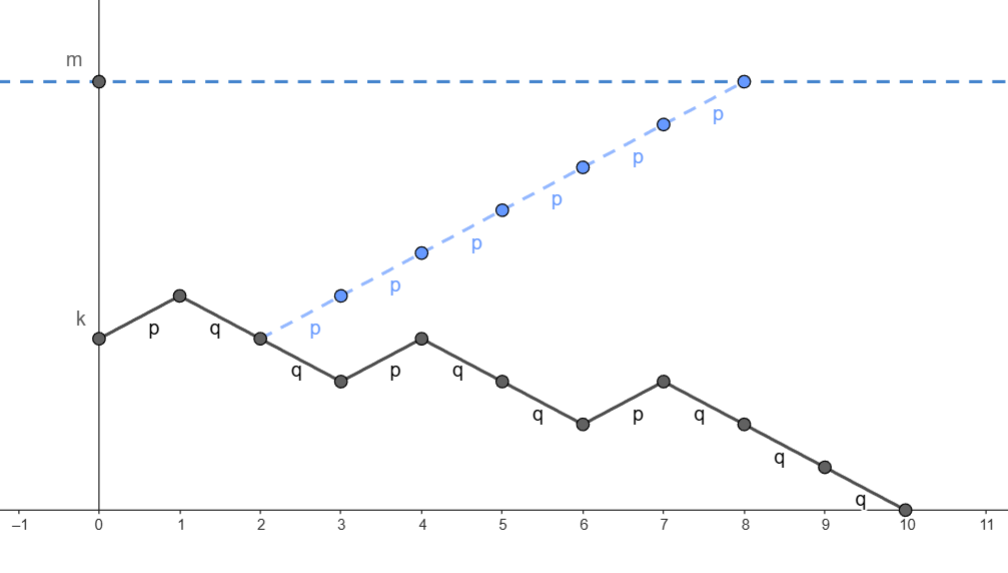
\includegraphics[height=7cm]{probtheory/images/probtheory_2024_10_15_1}
    \end{center}

    Пусть $r_k$ - интересующая нас вероятность разорение игрока при капитале $k$ (то есть достижения оси абсцисс на графике)

    $r_k = p \cdot r_{k + 1} + q r_{k - 1}$

    $pr_{k + 1} - r_k + (1 - p) r_{k - 1} = 0, \quad r_0 = 1, r_{m} = 0$

    $p\lambda^2 - \lambda + (1 - p) = 0$

    $D = 1 - 4p(1 - p) = 4p^2 - 4p + 1 = (2p - 1)^2$

    $\lambda_{1, 2} = \frac{1 \pm (2p - 1)}{2p}; \quad \lambda_1 = 1; \lambda_2 = \frac{2 - 2p}{2p} = \frac{q}{p}$

    Обозначим $\lambda = \frac{q}{p}$

    Рассмотрим два случая: 

    \begin{itemize}
        \item $p \neq \frac{1}{2}$

        Тогда общее решение: $r_k = C_1 \lambda_1^k + C_2 \lambda_2^k = C_1 + C_2 \lambda^k$

        Найдем частное решение:

        $\begin{cases}
            1 = C_1 + C_2 \\
            0 = C_1 + C_2 \lambda^m
        \end{cases} \Longleftrightarrow \begin{cases}
            C_1 = 1 - C_2 \\
            1 - C_2 + C_2 \lambda_m = 0
        \end{cases} \Longleftrightarrow \begin{cases}
            C_1 = 1 - C_2 \\
            C_2 (1 - \lambda_m) = 1
        \end{cases} \Longleftrightarrow \begin{cases}
            C_1 = 1 - \frac{1}{1 - \lambda^m} = \frac{-\lambda^m}{1 - \lambda^m} \\
            C_2 = \frac{1}{1 - \lambda^m}
        \end{cases}$

        $r_k = \frac{-\lambda^m}{1 - \lambda^m} + \frac{1}{1 - \lambda^m} \lambda^k = \frac{\lambda^k - \lambda^m}{1 - \lambda^m}$

        Посмотрим, что будет происходит при бесконечной игре (то есть когда $m \to \infty$ - капитал неограничен)

        1) $p < q$, то есть $\lambda > 1$. Тогда $\lambda^m \to \infty$, $r_k = \frac{\lambda^k - \lambda^m}{1 - \lambda^m} = \frac{\frac{\lambda^k}{\lambda_m} - 1}{\frac{1}{\lambda^m} - 1} \underset{n \to \infty}{\longrightarrow} 1$ - 
        то есть первый игрок гарантированно разорится

        2) $p > q$, то есть $\lambda < 1$. Тогда $\lambda^m \to 0$, $r_k = \frac{\lambda^k - \lambda^m}{1 - \lambda^m} \underset{n \to \infty}{\longrightarrow} \lambda^k$ - 
        то есть $r_k = \left(\frac{q}{p}\right)^k$

        \item $p = \frac{1}{2} \Longrightarrow D = 0$ 

        Тогда $\lambda_1 = \lambda_2 = 1$

        Общее решение: $r_k = C_1 \lambda^k + C_2 k \lambda_k = C_1 + C_2 k$

        Частное решение: 
        
        $\begin{cases}
            1 = C_1 \\
            0 = C_1 + C_2 m
        \end{cases} \Longleftrightarrow \begin{cases}
            1 = C_1 \\
            -1 = C_2 m
        \end{cases} \Longleftrightarrow \begin{cases}
            1 = C_1 \\
            C_2 = -\frac{1}{m}
        \end{cases}$

        $r_k = 1 - \frac{k}{m}$

        При бесконечной игре:

        $r_k = 1 - \frac{k}{m} \underset{m \to \infty}{\longrightarrow} 1$ - то есть при равной игре игрок неминуемо разорится 

    \end{itemize}

    \subsection{Случайное блуждание на прямой}

    Пусть в начальный момент времени находимся в начале координат. С вероятностью $p$ идем на единицу вправо, с вероятностью $q$ - влево

    При $p = \frac{1}{2}$ мы рано или поздно попадем в любую точку числовой прямой

    Можно привести аналогию с орлянкой: рано или поздно каждый игрок будет при сколь угодно большом выигрыше

    Посмотрим на орлянку как на распределение Бернулли:

    \smallvspace

    \begin{tabular}{c|c|c}
        $\xi$ & $-1$        & $1$    \\
        \hline
        $p$   & $\frac{1}{2}$ & $\frac{1}{2}$
    \end{tabular}

    \smallvspace

    $E\xi = 0; \quad D\xi = 1$

    Пусть $\xi$ - выигрыш первого после $n$ игр.

    $E\xi = \sum_{i = 1}^n E\xi_i = 0$

    $D\xi = \sum_{i = 1}^n D\xi_i = n$

    $\sigma_\xi = \sqrt{n}$ - среднее квадратическое отклонение

    Это означает, что при большом $n$ СКО поглотит всю числовую прямую

    $\frac{S_n}{n} \to E\xi$

    Закон больших чисел в этой ситуации говорит, что точка останется у 0, однако в то же время она может оказаться на любой точке на числовой прямой

    \Ex По $n$ конвертам случайным образом раскладывается $m$ писем. Случайная величина $\xi$ - число писем в своих конвертах

    $\letsymbol A_i$ - число $i$ письма в своем конверте, $\xi_i = I_A = \begin{cases}0, \quad i\text{-ое письмо в не своем конверте} \\ 1, \quad i\text{-ое письмо в своем конверте} \end{cases}$

    $\xi = \sum_{i = 1}^n \xi_i$

    $E\xi_i = P(A_i) = \frac{1}{n}$

    $D\xi_i = pq = \frac{1}{n} (1 - \frac{1}{n}) = \frac{n - 1}{n^2}$

    $E\xi = \sum_{i = 1}^n E\xi_i = 1 \frac{1}{n} = 1$ - в среднем будет одно письмо в своем конверте

    $D\xi = D(\xi_1 + \dots + \xi_n) = \sum_{i = 1}^n D\xi_i + 2\sum_{i < j} \mathrm{cov} (\xi_i, \xi_j)$

    Найдем ковариацию:

    $\mathrm{cov}(\xi_i, \xi_j) = E\xi_i \xi_j - E\xi_i E\xi_j = \frac{1}{n(n - 1)} - \frac{1}{n}\frac{1}{n} = \frac{n - (n - 1)}{n^2(n - 1)} = \frac{1}{n^2(n - 1)}$

    Заметим, что для любых $i, j, i < j$: $\xi_i \xi_j = \begin{cases}0, \quad \text{если хотя бы одно не в своем} \\ 1, \quad \text{если оба в своем}\end{cases}$
    
    То есть $\xi_i\xi_j \in B_p$ и $E\xi_i \xi_j = P(\text{оба письма в своих}) = \frac{1}{n(n - 1)}$

    Получаем: $D\xi = n \frac{n - 1}{n^2} + 2\frac{n(n - 1)}{2}\frac{1}{n^2(n - 1)} = \frac{n - 1}{n} + \frac{1}{n} = 1$

    



    

\end{document}
